%!TEX root = main.tex

\section{Appendix}

\subsection{Undecidability of $\strline$}

\noindent {\bf Proposition~\ref{prop-und}}.
{\it The path feasibility problem of $\strline$ is undecidable}.

\begin{proof}
The proof of Proposition~\ref{prop-und} is obtained by an encoding of post correspondence problem (PCP).
Let $\Sigma$ be a finite alphabet such that $\# \not\in \Sigma$ and $[n] \cap \Sigma = \emptyset$, $(u_i, v_i)_{i \in [n]}$ be a PCP instance with $u_i, v_i \in \Sigma^\ast$. A solution of the PCP instance is a string $i_1 \cdots i_m$ with $i_j \in [n]$ for every $j \in [m]$ such that $u_{i_1} \cdots u_{i_m} = v_{i_1} \cdots v_{i_m}$. We will use $\replaceall$ to encode the generation of the strings $u_{i_1} \cdots u_{i_m}$ and $v_{i_1} \cdots v_{i_m}$ from $i_1 \cdots i_m$, then use a regular expression with  capturing groups and back references to verify the equality of $u_{i_1} \cdots u_{i_m}$ and $v_{i_1} \cdots v_{i_m}$. Specifically, suppose $\# \not \in \Sigma$, then the PCP instance is encoded by the following $\strline$ program,
\[
\begin{array}{l}
\ASSERT{x_0 \in \{1, \cdots, n\}^+}; \\
x_1 := \replaceall_{1, u_1}(x_0); \cdots; x_n:=\replaceall_{n, u_n}(x_{n-1}); \\
y_1:=\replaceall_{1, v_1}(x_0); \cdots; y_n:=\replaceall_{n, u_n}(y_{n-1});\\
z:= x_n \# y_n; \ASSERT{z \in (\Sigma^+)\#\$1}.
\end{array}
\]
\end{proof}

% \subsection{Proof for Theorem \ref{theorem:regex_pnfa_equiv}}
% 
% \label{proof:regex_pnfa_equiv}
% 
% We restate the theorem here:
% \begin{theorem}
%   For any regular expression e, subexpression $e'$ of e, and $w \in L (e)$,
%   $m_{e', e} (w) = p_{e', e} (w)$
% \end{theorem}
% 
% \begin{proof}
%   We first observe the fact that when $e' = e$, we have $m_{e', e} (w) =
%   p_{e', e} (w) = w$. Therefore, we suppose $e' \neq e$ in the following
%   argument.
%   
%   We perform induction on $e$:
%   \begin{itemize}
%     \item The base case, when $e = \varepsilon$ or $e = a$, is routine and
%     trivial.
%     
%     \item If $e = (e_1)$, then for any $w \in L (e)$, we have $w \in L (e_1)$,
%     and for any subexpression $e' \neq e$, $e'$ is also a subexpression of
%     $e_1$. By induction, \ $m_{e', e_1} (w) = p_{e', e_1} (w)$. Because $A_e =
%     A_{e_1}$, $p_{e', e_1} (w) = p_{e', e} (w)$. By definition of match tree,
%     we also have $m_{e', e_1} (w) = m_{e', e} (w)$. Thus $m_{e', e} (w) =
%     p_{e', e} (w)$.
%     
%     \item If $e = e_1 + e_2$, then for any $w \in L (e)$, either $w \in L
%     (e_1)$ or $w \in L (e_2)$. Also, any subexpression $e' \neq e$ is a
%     subexpression of either $e_1$ or $e_2$.
%     
%     If $w \in L (e_1)$, then if $e'$ is a subexpression of $e_2$, we have
%     $m_{e', e} (w) = p_{e', e} (w) = \emptyset$, otherwise by induction we
%     have $m_{e', e_1} (w) = p_{e', e_1} (w)$. Suppose $p = q_0 \sigma_1 q_1
%     \ldots \sigma_m q_m$ is the accepting run of $A_{e_1}$, then by definition
%     of $A_e$, we know p is also the accepting run of $A_e$, thus $p_{e', e_1}
%     (w) = p_{e', e} (w)$. By definition of match tree, we have $m_{e', e_1}
%     (w) = m_{e', e} (w)$. Thus $m_{e', e} (w) = p_{e', e} (w)$.
%     
%     Similarly, when $w \in L (e_2)$, we also have $m_{e', e} (w) = p_{e', e}
%     (w)$.
%     
%     \item If $e = e_1 e_2$, then for any $w \in L (e)$, suppose $w = w_1 w_2$
%     such that $C (m_e (w)) = (w_1, e_1) (w_2, e_2)$.
%     
%     Assuming $p = q_0 \sigma_1 q_1 \ldots \sigma_m q_m$ is the accepting run
%     of $A_e$ on w, and $w_1 = \sigma_1 \ldots \sigma_i$, $w_2 = \sigma_{i + 1}
%     \ldots \sigma_m$, we know $q_0 \sigma_1 q_1 \ldots \sigma_i q_i$ is the
%     accepting run of $A_{e_1}$ on $w_1$. If not, suppose the accepting run of
%     $A_{e_1}$ on $w_1$ is $q_0 \sigma_1' q_1' \ldots \sigma_i' q_i'$ instead,
%     then by definition of $A_e$, another run of $A_e$ on
%     w, $q_0 \sigma_1' q_1' \ldots \sigma_i' q_i'
%     \sigma_{i + 1} q_{i + 1} \ldots \sigma_m q_m$, is of higher priority than p, which leads to contradiction.
%     Similarly, we know $q_0 \sigma_{i + 1} q_{i + 1} \ldots \sigma_m q_m$ is
%     the accepting run of $A_{e_2}$ on $w_2$.
%     
%     If $e'$ is a subexpression of $e_1$, then by induction, $m_{e', e_1} (w_1)
%     = p_{e', e_1} (w_1)$. By definition of match tree, $e'$ cannot occur in
%     the subtree $(w_2, e_2)$, thus we have $m_{e', e_1} (w_1) = m_{e', e}
%     (w)$. Because the maximal $e'$-matches in p only occur in $q_0 \sigma_1
%     q_1 \ldots \sigma_i q_i$, we also have $p_{e', e_1} (w_1) = p_{e', e}
%     (w)$. Thus $m_{e', e} (w) = p_{e', e} (w)$.
%     
%     Similarly when $e'$ is a subexpression of $e_2$, we have $m_{e', e} (w) =
%     p_{e', e} (w)$.
%     
%     \item If $e = e_1^{\ast}$, then for any $w \in L (e)$, if $w =
%     \varepsilon$ it is obvious that $m_{e', e} (w) = p_{e', e} (w) =
%     \emptyset$ for any $e'$. Otherwise, suppose $w = w_1 \ldots w_n$ such that
%     $C (m_e (w)) = (w_1, e_1) \ldots (w_n, e_1)$.
%     
%     Assuming $p = q_0 \sigma_1 q_1 \ldots \sigma_m q_m$ is the accepting run
%     of $A_e$ on w, $w_1 = \sigma_1 \ldots \sigma_{i_1}$, $w_2 = \sigma_{i_1 +
%     1} \ldots \sigma_{i_2}$ .etc, and $w_n = \sigma_{i_{m - 1} + 1} \ldots
%     \sigma_m$, we know $p_k = q_0 \sigma_{i_{k - 1} + 1} q_{i_{k - 1} + 1}
%     \ldots \sigma_{i_k} q_{i_k}$ is the accepting run of $A_{e_1}$ on
%     $w_k$. The proof is similar to the one above when $e = e_1 e_2$, and we
%     will omit it for simplicity.
%     
%     For any subexpression $e'$ of $e_1$, by induction, we have $m_{e', e_1}
%     (w_k) = p_{e', e_1} (w_k)$ for all $k \in [n]$. By definition of match
%     tree, we have $m_{e', e} (w) = m_{e', e_1} (w_1) \ldots m_{e', e_1}
%     (w_n)$. Because all the maximal $e'$-matches in p only occur in $p_k$ for
%     some $k \in [n]$ (that is, all the states in a $e'$-matches occur in the
%     same segment of $p$), we also have $p_{e', e} (w) = p_{e', e_1} (w_1)
%     \ldots p_{e', e_1} (w_n)$. Thus $m_{e', e} (w) = p_{e', e} (w)$.
%   \end{itemize}
% \end{proof}


\subsection{From $\cgexp$ to PFA}

For any $e \in \cgexp$, a PFA $\cA_e$ is constructed recursively in the sequel. The constructed PFA $\cA_e$ satisfies that it has a unique initial state and a unique final state  without outgoing transitions.
%The original construction on regular expressions
%produces an FA without $\varepsilon$-transitions, which we denote by $G_e$.
%We refer the reader to \cite{Gluskov61} for 
%details of how to construct $G_e$. %\tl{is this just the textbook construction?}
%
%The pNFA $A_e$ is obtained by recursively adding priority to $G_e$ as follows:
\begin{itemize}
\item If $e =\emptyset$, then $\cA_e = (\{q_0,f_0\}, \Sigma, \delta, \tau, q_0, f_0)$, where $\delta(q_0, \sigma) = \delta(f_0, \sigma) = ()$ for every $\sigma \in \Sigma$, $\tau(q_0) = \tau(f_0)= ((); ())$.

  \item If $e = \varepsilon$, then  $\cA_e = (\{q_0, f_0\}, \Sigma, \delta, \tau, q_0, f_0)$, where  $\delta(q_0, \sigma) = \delta(f_0, \sigma) = ()$ for every $\sigma \in \Sigma$, $\tau(q_0) = ((f_0); ())$, and $\tau(f_0) = ((); ())$. 

  \item If $e = a$, then $\cA_e = (\{q_0, f_0\}, \Sigma, \delta, \tau, q_0, f_0)$, where  $\delta(q_0, a) = (f_0)$, $\delta(q_0, \sigma) = ()$ for every $\sigma \in \Sigma \setminus \{a\}$, $\tau(q_0) = ((); ())$, and $\tau(f_0) = ((); ())$.
    
  \item If $e = (e_1)$, then $\cA_e = \cA_{e_1}$.
  
  \item If $e = e_1 + e_2$, and suppose $\cA_{e_1} = (Q_1,
  \Sigma, \delta_1, \tau_1, q_1, f_1)$ and $\cA_{e_2} = (Q_2, \Sigma,
  \delta_2, \tau_2, q_2, f_2)$, then $\cA_e = (Q_1 \cup Q_2 \cup \{q_0, f_0\}, \Sigma,
  \delta, \tau, q_0, f_0)$, where  
  \begin{itemize}
 \item $q_0, f_0 \not \in Q_1 \cup Q_2$, 
 \item $\delta(q) = \delta_i(q)$ for every $q \in Q_i$ ($i=1,2$), 
$\delta(q_0, \sigma) = \delta(f_0, \sigma) = ()$ for every $\sigma \in \Sigma$, 
%
 \item $\tau(q) = \tau_i(q)$ for every $q \in Q_i$ ($i =1,2$), $\tau(q_0) = ((q_1,q_2); ())$,  $\tau(f_1) = \tau(f_2) = ((f_0); ())$, and $\tau(f_0) = ((); ())$.
 \end{itemize}
%
  \item If $e = e_1 \concat e_2$, and suppose $\cA_{e_1} = (Q_1,
  \Sigma, \delta_1, \tau_1, q_1, f_1)$ and $\cA_{e_2} = (Q_2, \Sigma,
  \delta_2, \tau_2, q_2, f_2)$, then $\cA_e = ( Q_1 \cup Q_2, \Sigma, \delta, \tau, q_1,
  f_2)$, where 
  \begin{itemize}
    \item for every $q \in Q_i$, $\delta(q) = \delta_i(q)$ ($i = 1,2$),
    
    \item for every $q \in Q_2$, $\tau(q) = \tau_2(q)$, 
%
    \item for every $q \in Q_1 \setminus \{f_1\}$, $\tau(q) = \tau_1(q)$, and $\tau(f_1) = ((q_2); ())$.
  \end{itemize}
%  
  \item If $e = e_1^{\ast}$, and suppose  $\cA_{e_1} = (Q_1,
  \Sigma, \delta_1, \tau_1, q_1, f_1)$, then $\cA_e = (Q_1 \cup \{f_0\}, \Sigma,
  \delta, \tau, q_1, f_0)$, where 
  \begin{itemize}
  \item $f_0 \not \in Q_1$,
  
    \item for every $q \in Q_1$ and $\sigma \in \Sigma$, $\delta(q, \sigma) = \delta_1(q, \sigma)$, 
    %moreover, $\delta(q_0, \sigma) = \delta(f_0, \sigma)  = ()$,
    
    \item for every $q \in Q_1 \setminus \{q_1, f_1\}$,  $\tau(q) = \tau_1(q)$, moreover, $\tau(q_1) = (\pi_1(\tau_1(q_1)); (\pi_2(\tau_1(q_1)), f_0))$, $\tau(f_1) = ((q_1); ())$, and $\tau(f_0) = ((); ())$. (Intuitively, the $\varepsilon$-transitions from $f_1$ to $q_1$ and from $q_1$ to $f_0$ respectively are added, moreover, the $\varepsilon$-transition from $q_1$ to $f_0$ is of the lowest priority.)
  \end{itemize}
 %
  \item If $e = e_1^{\ast?}$, and suppose $\cA_{e_1} = (Q_1,
  \Sigma, \delta_1, \tau_1, q_1, f_1)$, then $\cA_e = (Q_1 \cup \{f_0\}, \Sigma,
  \delta, \tau, q_1, f_0)$, where 
  \begin{itemize}
  \item $q_0, f_0 \not \in Q_1$,
  
    \item for every $q \in Q_1$ and $\sigma \in \Sigma$, $\delta(q, \sigma) = \delta_1(q, \sigma)$, 
    %moreover, $\delta(q_0, \sigma) = \delta(f_0, \sigma)  = ()$,
    
    \item for every $q \in Q_1 \setminus \{q_1, f_1\}$,  $\tau(q) = \tau_1(q)$, moreover, $\tau(q_1) = ((f_0, \pi_1(\tau_1(q_1))); \pi_2(\tau_1(q_1)))$, $\tau(f_1) = ((q_1); ())$, and $\tau(f_0) = ((); ())$. (The $\varepsilon$-transition from $q_1$ to $f_0$ is of the highest priority.)
  \end{itemize}  
\end{itemize}

%The key transitions of some non-trivial cases of the construction are illustrated in Figure.\ref{fig:pglushkov}.

% An important property of the automaton $G_e$ and thus $A_e$ is that, for any subexpression $e'$ of $e$, there must be a subgraph of $A_{e}$ corresponding to $e'$. We denote this subgraph by $A_{e}[e']$. This subgraph can be seen as the automaton obtained by removing from $A_{e'}$ the state $q_0$ and all transitions from it.

\begin{example}
Let $e_1 = a^\ast$ and $e_2 = a^{\ast ?}$. Then the PFAs $\cA_{e_1} = (Q_1, \Sigma, \delta_1, \tau_1, q_0, q_3)$ and $\cA_{e_2} =  (Q_2, \Sigma, \delta_2, \tau_2, q_0, q_3)$ are illustrated in Figure~\ref{fig-retopfa}: (i), (ii), where thicker solid lines (resp. dashed lines) denote the $\varepsilon$-transitions of higher (resp. lower) priorities than non-$\varepsilon$-transitions. For instance, in $\cA_{e_1}$, $\tau_1(q_0) = ((); (q_2))$ and $\tau_1(q_1) = ((q_0); ())$, while in $\cA_{e_2}$, $\tau_2(q_0) = ((q_2); ())$ and $\tau_2(q_1) = ((q_0); ())$. Note that $\cA_{e_1}$ and $\cA_{e_2}$ are slightly different from those in Example~\ref{exmp-pfa}.
\begin{figure}[ht]
\centering
%\rule{\linewidth}{0cm}
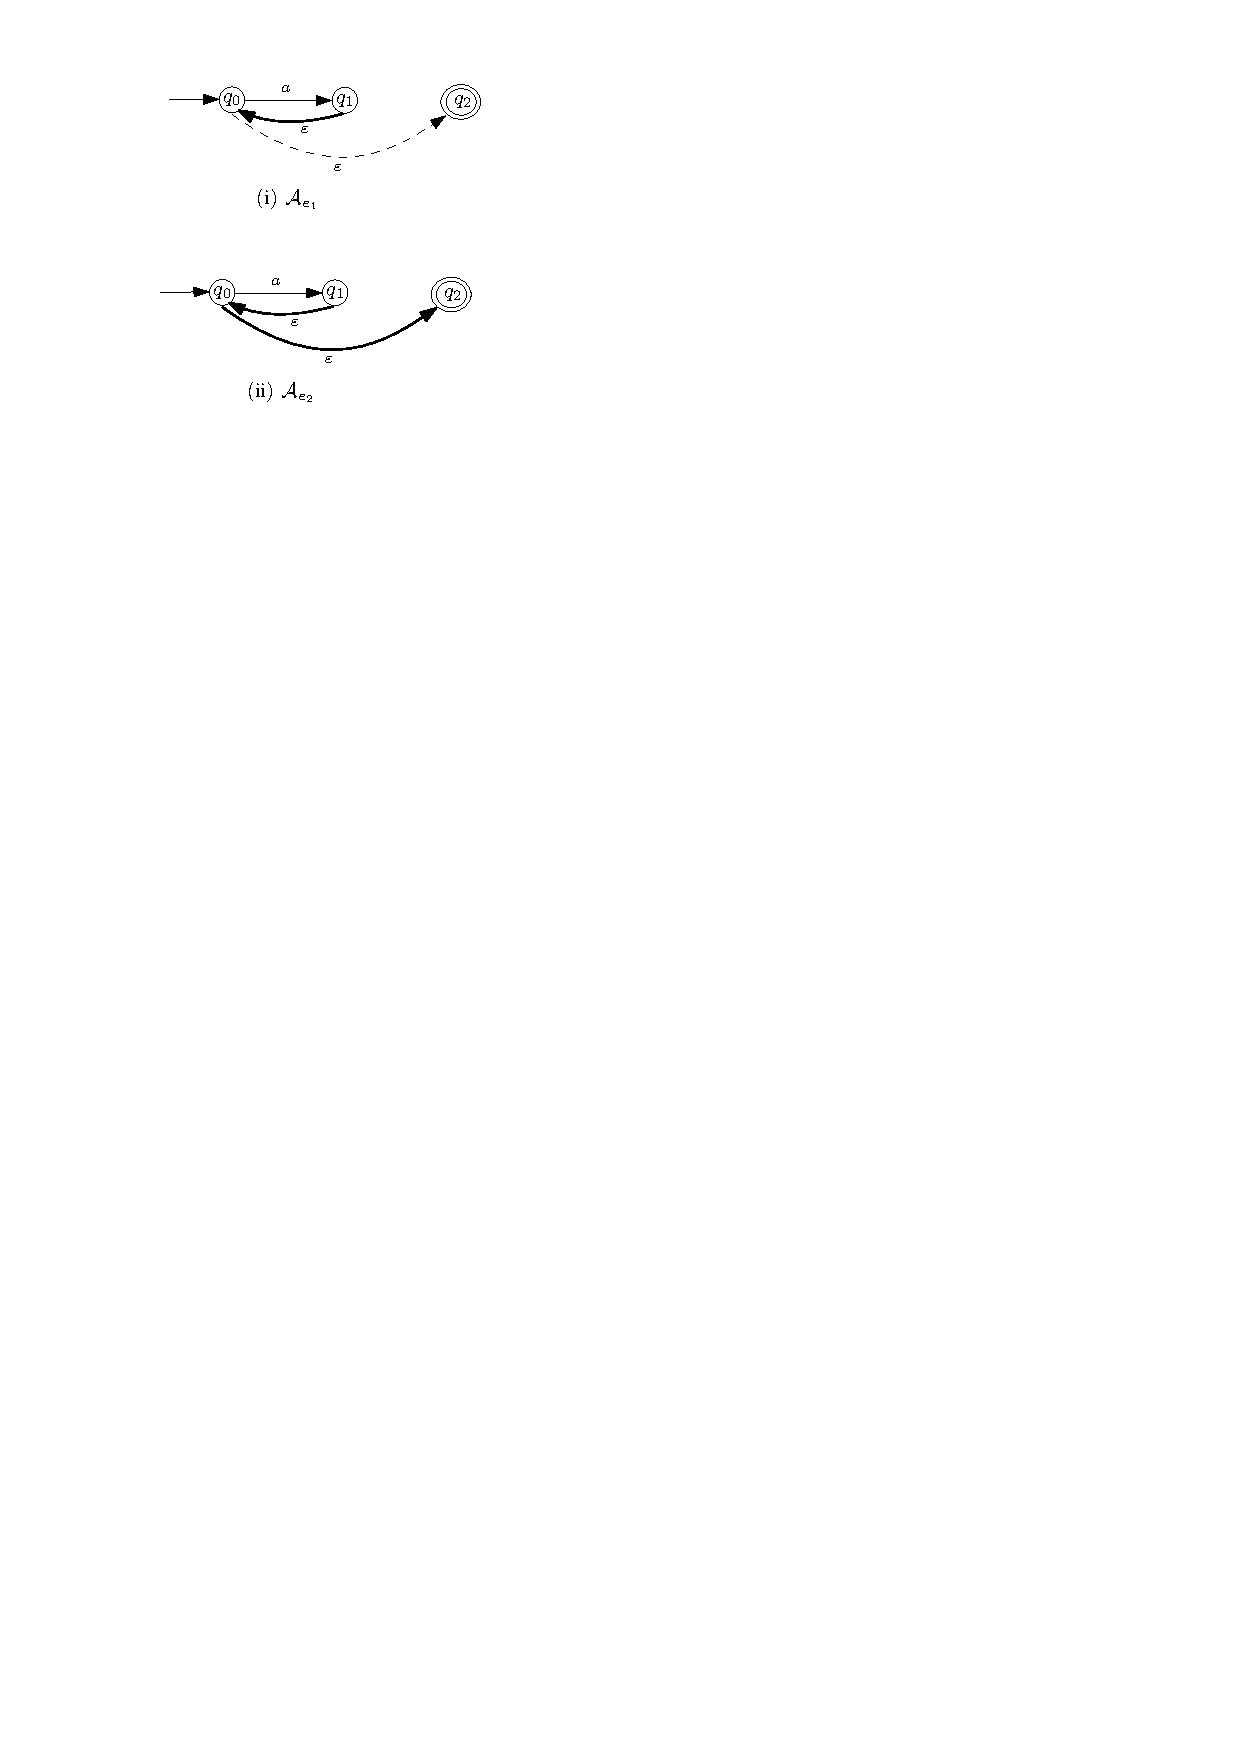
\includegraphics[scale=0.8]{retopfa.pdf}
\caption{$\cA_{e_1}$ and $\cA_{e_2}$ for $e_1= a^\ast$ and $e_2 = a^{\ast?}$}
\label{fig-retopfa}
\end{figure}
\end{example}
 

